% VLDB template version of 2020-08-03 enhances the ACM template, version 1.7.0:
% https://www.acm.org/publications/proceedings-template
% The ACM Latex guide provides further information about the ACM template

\documentclass[sigconf, nonacm]{acmart}

% By Jialun Shen
\usepackage{algorithm}
\usepackage{algorithmic}
\usepackage{amssymb}
\usepackage{amsthm}
\usepackage{amsmath}
\usepackage{bm}
\usepackage{framed}
\usepackage{graphicx}
\newcommand*{\algorithmautorefname}{Algorithm}

%% The following content must be adapted for the final version
% paper-specific
\newcommand\vldbdoi{XX.XX/XXX.XX}{}
\newcommand\vldbpages{XXX-XXX}
% issue-specific
\newcommand\vldbvolume{14}
\newcommand\vldbissue{1}
\newcommand\vldbyear{2021}
% should be fine as it is
\newcommand\vldbauthors{\authors}
\newcommand\vldbtitle{\shorttitle}
% leave empty if no availability url should be set
\newcommand\vldbavailabilityurl{https://github.com/sgallon-rin/graph-data-final}
% whether page numbers should be shown or not, use 'plain' for review versions, 'empty' for camera ready
\newcommand\vldbpagestyle{plain} 

\begin{document}
\title{Efficient Reduction Rules for Calculating Near-maximum Weighted Independent Set}

%%
%% The "author" command and its associated commands are used to define the authors and their affiliations.
\author{Jialun Shen}
\author{Ruifan Deng}
\affiliation{%
  \institution{Fudan University}
  \streetaddress{220 Handan Road}
  \city{Shanghai}
  \state{China}
  \postcode{200433}
}
\email{16307110030@fudan.edu.cn}
\email{18300180053@fudan.edu.cn}

%%
%% The abstract is a short summary of the work to be presented in the
%% article.
\begin{abstract}
% TODO: abstract
Cras fermentum facilisis elit vitae egestas. Mauris porta, neque non rutrum efficitur, odio odio faucibus tortor, vitae imperdiet metus quam vitae eros. Proin porta dictum accumsan. Aliquam dapibus a velit. Curabitur vitae nulla dapibus, ornare dolor in, efficitur enim. Ut maximus mi id arcu ultricies feugiat. Phasellus facilisis purus ac ipsum varius bibendum.
Cras fermentum facilisis elit vitae egestas. Mauris porta, neque non rutrum efficitur, odio odio faucibus tortor, vitae imperdiet metus quam vitae eros. Proin porta dictum accumsan. Aliquam dapibus a velit. Curabitur vitae nulla dapibus, ornare dolor in, efficitur enim. Ut maximus mi id arcu ultricies feugiat. Phasellus facilisis purus ac ipsum varius bibendum.
Cras fermentum facilisis elit vitae egestas. Mauris porta, neque non rutrum efficitur, odio odio faucibus tortor, vitae imperdiet metus quam vitae eros. Proin porta dictum accumsan. 
\end{abstract}

\maketitle

%%% do not modify the following VLDB block %%
%%% VLDB block start %%%
\pagestyle{\vldbpagestyle}
\begingroup\small\noindent\raggedright\textbf{PVLDB Reference Format:}\\
\vldbauthors. \vldbtitle. PVLDB, \vldbvolume(\vldbissue): \vldbpages, \vldbyear.\\
\href{https://doi.org/\vldbdoi}{doi:\vldbdoi}
\endgroup
\begingroup
\renewcommand\thefootnote{}\footnote{\noindent
This work is licensed under the Creative Commons BY-NC-ND 4.0 International License. Visit \url{https://creativecommons.org/licenses/by-nc-nd/4.0/} to view a copy of this license. For any use beyond those covered by this license, obtain permission by emailing \href{mailto:info@vldb.org}{info@vldb.org}. Copyright is held by the owner/author(s). Publication rights licensed to the VLDB Endowment. \\
\raggedright Proceedings of the VLDB Endowment, Vol. \vldbvolume, No. \vldbissue\ %
ISSN 2150-8097. \\
\href{https://doi.org/\vldbdoi}{doi:\vldbdoi} \\
}\addtocounter{footnote}{-1}\endgroup
%%% VLDB block end %%%

%%% do not modify the following VLDB block %%
%%% VLDB block start %%%
\ifdefempty{\vldbavailabilityurl}{}{
\vspace{.3cm}
\begingroup\small\noindent\raggedright\textbf{PVLDB Artifact Availability:}\\
The source code, data, and/or other artifacts have been made available at \url{\vldbavailabilityurl}.
\endgroup
}
%%% VLDB block end %%%

\section{Introduction}

The maximum independent set (short as MIS) of a graph $G$ is the largest vertex set $S$, where each two vertices are non-adjacent, in $G$. It is a classic NP-hard problem in graph theory that has attracted much attention~\cite{lewis1983computers}. However, the traditional MIS problem does not take vertex weight into consideration. Vertex weight can have very important information. In real-world graphs, the vertices do not equally contribute to the MIS.

% TODO: example?
% For example, 

The maximum weighted independent set (short as MWIS) of a weighted graph $G$ is the independent set with largest total weight, which has a wide-range of practical applications in many areas such as map labeling, alignment of biological networks, wireless communication and so on~\cite{gellner2021boosting}. In MWIS, the weight of an independent set is the sum of weights of all the vertices in $S$. When all the vertices are identical, the computation of MWIS is the same as the computation of MIS. As a result, computing MWIS is also a NP-hard problem and the existing algorithms designed for computing MIS can not be used to solve MWIS problem directly.

We notice that the reduction-based algorithms behave very efficiently when being applied to reduce the size of graph while the correctness of the results is preserved~\cite{fomin2009measure,chang2017computing}. The main idea is to determine whether the vertices are definitely in MIS. However, the reduction rule devised for unweighted graphs cannot be used to compute MWIS on weighted graphs. Based on related works, we focus on designing new reduction rules for general weighted graphs. Inspired by single-vertex reduction and two-vertex reduction~\cite{Zheng:2020aa}, we propose k-vertex reduction. When no reduction rules can be applied, a heuristic strategy is adopted to delete a vertex from the current graph until one reduction rule can be used.

\section{Problem Definition}

In the following definitions, the graph $G$ refers to an undirected vertex-weighted graph $G(V,E,\omega)$ with weight function $\omega: V\to\mathbb{R}^+$, without further specification. Let $V_G$ denote the set of vertices in $G$, $E_G$ denote the set of edges in $G$. In such a graph $G$, weight of an independent set canbe defined, which turns it into a weighted independent set. Note that we do not consider edge weights, which can be omitted when computing an independent set or a weighted independent set.

\begin{framed}
\noindent\textbf{Definition 2.1:} (\emph{Independent Set}). 

An independent set $IS(G)$ is a set of vertices in a graph $G$, no two of which are adjacent. Its size $|IS(G)|$ is the number of vertices in it.

\noindent\textbf{Definition 2.2:} (\emph{Weight of an Independent Set}). 

The weight of $IS(G)$, denoted by $\omega(IS(G))$, is the sum of the weights of the vertices in $IS(G)$, i.e., $\omega(IS(G)) = \sum_{u\in IS(G)}\omega(u)$.

\noindent\textbf{Definition 2.3:} (\emph{Maximal Independent Set}). 

A maximal independent set is an independent set that is not a proper subset of any other independent set. 

\noindent\textbf{Definition 2.4:} (\emph{Maximum Independent Set}). 

A maximum independent set, denoted by $MIS(G)$, is an independent set of largest possible size for a given graph $G$.

\noindent\textbf{Definition 2.5:} (\emph{Maximum Weighted Independent Set}). 

Given a graph $G$, a maximum weighted independent set, denoted by $MWIS(G)$, is an $IS(G)$ with the largest weight.
\end{framed}

Computing the exact $MWIS(G)$ is a non-trivial task. Thus, it is usually acceptable to compute a near-optimal weighted independent set in real-world applications.

\section{Related Work}

\subsection{Exact Algorithms}

Exact algorithms usually compute optimal solutions by systematically exploring the solution space. A frequently used paradigm in exact algorithms for combinatorial optimization problems is called branch-and-bound~\cite{ostergaard2002fast,warren2006combinatorial}. For the MWIS problem, these types of algorithms compute optimal solutions by case distinctions in which vertices are either included into the current solution or excluded from it, branching into two or more subproblems and resulting in a search tree. There have been many research to improve exact branch-and-bound algorithms. These improvements include different pruning methods and complicated branching schemes with upper and lower bounds to exclude specific subtrees. \citet{warren2006combinatorial} proposed three branch-and-bound algorithms which combine the use of weighted clique covers and a branching scheme introduced by~\citet{balas1986finding}. Their algorithms are able to quickly solve instances with hundreds of vertices.

In recent years, reduction rules have frequently been added into branch-and-bound methods yielding the branch-and-reduce algorithms. These algorithms are able to improve the worst case runtime of branch-and-bound algorithms by applying the reduction rules to the current graph before each branching step~\cite{fomin2009measure}. Specifically, two cases should be considered for a vertex $u$: $u$ is included in the MWIS, or $u$ is not included in the MWIS. In the first case, all neighbors of $u$ cannot belong to the MWIS. The Algorithm is recursively invoked to compute the maximum weighted independent set $S$ of $G\backslash(\{u\} \cup N(u))$, where $N(u)$ is the set of neighbors of $u$ and $G\backslash R$ represents the graph remained by removing the vertices in the vertex set $R$ and the incident edges. If it holds that $\omega(u)+\omega(S)>\max W$, we use $S\cup\{u\}$ to update $MWIS(G)$. In the second case, the process is recursively invoked to compute the maximum weighted independent set $S$ of $G\backslash\{u\}$. If its weight is larger than $\max W$, the MWIS is updated with $S$.

\subsection{Heuristic Algorithms}

A widely used heuristic approach is local search, which usually computes an initial solution and then improves it by simple insertion, removal or swap operations. Although local search generally cannot guarantee the solution’s quality theoretically, in practice they find high quality solutions significantly faster than exact procedures. Moreover, heuristic algorithms for the minumim weighted vertex cover problem~\cite{2018Improving,2017An} can be helpful to solve the MWIS problem, as vertex cover and independent set are two complementary concepts in graphs.

\subsection{Hybrid Algorithms}

In order to overcome the drawbacks of both exact and inexact methods, new approaches combining reduction rules with heuristic local search algorithms were proposed~\cite{Lamm0SWZ19}. A very successful approach using this paradigm is the reducing-peeling framework. The algorithm works by computing a kernel using practically efficient reduction rules in linear and near-linear time. In addition, they provide an extension of their reduction rules that is able to compute good initial solutions for the kernel. In particular, they greedily select vertices that are unlikely to be in a large independent set, then opening up the reduction space again. Thus, they are able to significantly improve the performance of the local search algorithm that is applied on the kernelized graph.

\subsection{Near-Maximum WIS Computation}

Inspired by the reducing-and-peeling strategy, a greedy algorithm to compute a near-maximum weighted independent set is proposed. It first applies the reduction rules to add the vertices that must be contained in the $MWIS(G)$, and deletes their neighbors from $G$. When no reduction rules can be applied to the current graph, we need to delete some the largest-degree vertices so that at least one reduction rule becomes available. Actually, the greedy strategy follows the heuristic: removing the vertices that are less likely to be included in the $MWIS(G)$.

The greedy strategy offers no guarantees for deleting the vertices that cannot be included in the maximum weighted independent set. Actually, the key task is designing effective reduction rules to reduce the size of the input graph. Note that the reduction rules can be also applied to reduce the search space for algorithms that compute the exact MWIS. \citet{Zheng:2020aa} proposed the following three theorems. For ease of presentation, let $\omega(S)$ denote the sum of weights of all the vertices in the set $S$.

\begin{framed}
\noindent\textbf{Theorem 3.1:} (\emph{Single-Vertex Reduction}). 

Given a vertex $u\in G$ and its neighbors $N(u)$, if $\omega(u)\geq\omega(N(u))$, $u$ must be contained by one MWIS of $G$; thus the vertices in $N(u)$ can be removed, and it holds that $MWIS(G)=MWIS(G')\cup\{u\}$, where $G'= G\backslash(N(u)\cup u)$.

\noindent\textbf{Theorem 3.2:} (\emph{Two-Vertex Reduction}). 

Given two vertices $u, v\in G$ and their neighbors $P$, $u$ and $v$ must be contained by one MWIS of $G$ if it holds that: (1) $\omega(u)+\omega(v)\geq\omega(P)$; and (2) $\omega(x)<\omega(N(x))$ for each vertex $x\in\{u,v\}$. Thus the vertices in $P$ can be removed, and it holds that $MWIS(G)=MWIS(G')\cup\{u,v\}$, where $G'=G\backslash(P\cup\{u,v\})$.

\noindent\textbf{Theorem 3.3:}

Let $G$ be a graph obtained after applying single-vertex reduction. Each two vertices $u_1$ and $u_2$ must share one common neighbor at least if they are added into $MWIS(G)$ by the two-vertex reduction.
\end{framed}

Here, we provide the proof of Theorem 3.2 since it is omitted in the original paper~\cite{Zheng:2020aa}.

\begin{proof}
%\noindent\textbf{Proof:} 
When we consider a pair of nodes $(u, v)$, it implies that they do not belong to $S$ after applying single-vertex reduction. Thus, $\omega(u)<\omega(N(u))$ and $\omega(v)<\omega(N(v))$. Assume $u$ and $v$ do not belong to $S$ after applying two-vertex reduction, then let $P'$ be the MWIS in $P$, we have $\omega(u)+\omega(v)\geq\omega(P)\geq\omega(P')$. Therefore, we can replace $P'$ with $\{u, v\}$. %$\hfill\square$
\end{proof}

Since the single-vertex reduction is cheaper, it is always applied before the two-vertex reduction. Therefore, the input of two-vertex reduction is the remaining graph that is applied the single-vertex reduction before. Instead of enumerating all pairs of vertices, it just needs to examine the pairs of vertices $(u_1, u_2)$ that share one common neighbor at least.

When no reduction rules can be applied to the current graph, we need to delete some of the largest-degree vertices so that at least one reduction rule becomes available. The greedy strategy follows the heuristic: removing the vertices that are less likely to be included in the $MWIS(G)$.

\section{Our Work}

\subsection{Improvement of Reduction Algorithms}

Vertices with larger weights are more likely to be in the MWIS. If they do, check them earlier may prune their neighbors earlier, so that there will be less vertices to check in $V_G$. Therefore, prior to applying the reduction rules, sorting the vertices by weight in descending order can possibly be helpful. However, sorting the vertices brings extra cost, which is tested in our experiment.

\begin{algorithm}[tbp]
\caption{Two-vertex Reduction with Sort}
\label{alg:2vertexsort}
%\SetAlgoLined
\begin{algorithmic}
	\STATE   \textbf{Input} A graph $G=(V_G,E_G,\omega)$
        %\vspace*{-.45cm}
	\STATE   \textbf{Output} $S$: a set of vertices in $MWIS(G)$
	\STATE   initialize $S\leftarrow \emptyset$
	\STATE   \textbf{for} each vertex $u\in V_G$ \textbf{do}
	\STATE   \quad $T \leftarrow \emptyset$
	\STATE   \quad \textbf{for} each vertex $v\in N(u)$ \textbf{do}
	\STATE   \quad \quad \textbf{for} each vertex $w\in N(v)$ \textbf{do}
	\STATE   \quad \quad \quad \textbf{if} $e(u,w) \notin E_G$ \textbf{then}
	\STATE   \quad \quad \quad \quad $T \leftarrow T \cup \{w\}$
	\STATE   \quad calculate the maximal independent sets $\mathcal{M}=\{M_1,...,M_a\}$, $M_i \subseteq T$, $i=1,...,a$
	\STATE   \quad sort $\mathcal{M}$ in descending order so that $\omega(M_1)\geq...\geq\omega(M_a)$
	\STATE   \quad \textbf{for} $M_i\in\mathcal{M}$ \textbf{do}
	\STATE   \quad \quad \textbf{if} $\omega(u)+\omega(M_i)\geq \omega(N(u)\cup N(M_i))$ \textbf{then}
	\STATE   \quad \quad \quad $S\leftarrow S\cup\{u\}\cup M_i$
	\STATE   \quad \quad \quad remove $\{u\}$, $M_i$ and $N(u)\cup N(M_i)$ from G
	\STATE   \quad \quad \quad \textbf{break}
\end{algorithmic}
\end{algorithm}

\subsection{Generalization of the Reduction Rule}

On the basis of theorem 3.1 and 3.2, we generalized it to k-vertex reduction as the following theorem:

\begin{framed}
\noindent\textbf{Theorem 4.1:} (\emph{$k$-Vertex Reduction}). 

Given a  set of vertices $\{u_1, u_2, \cdots, u_k\}\in G$ and their neighbors $P=\bigcup_{i=1}^nN(u_i)$, $\{u_1, u_2, \cdots, u_k\}$ must be contained by a MWIS of G if it holds that: (1) $\omega(u_1) + \omega(u_2) + \cdots + \omega(u_k) \geq \omega(P)$; and (2) $\omega(x) < \omega(N(x))$ for each vertex $x\in\{u_1, u_2, \cdots, u_k\}$. Thus the vertices in $P$ can be removed, and it holds that $MWIS(G) = MWIS(G')\cup\{u_1, u_2, \cdots, u_k\}$, where $G'=G\backslash (P\cup\{u_1, u_2, \cdots, u_k\}), k \geq 2$.
\end{framed}

\begin{proof}
When we consider a set of $k$ vertices $\{u_1, u_2, \cdots, u_k\}$, it implies that they do not belong to $S$ after applying single-vertex to $(k-1)$-vertex reduction. Thus, $\omega(u_i)<\omega(N(u_i))$ for all $i\in\{1,2,\cdots,k\}$. Assume $u_1, u_2, \cdots, u_k$ do not belong to $S$ after applying $k$-vertex reduction, then let $P'$ be the MWIS in $P$, we have $\sum_{i=1}^k\omega(u_i)\geq\omega(P)\geq\omega(P')$. Therefore, we can replace $P'$ with $\{u_1, u_2, \cdots, u_k\}$.
\end{proof}

For a graph after applying $(k-1)$-vertex reduction, it has the following properties, given in theorem 4.2 and 4.3.

\begin{framed}
\noindent\textbf{Theorem 4.2:}

Let $G$ be a graph obtained after applying $(k-1)$-vertex reduction. Each set of $k$ vertices $\{u_1, u_2, \cdots, u_k\}$ must share one common neighbor at least if they are added into $MWIS(G)$ by $k$-vertex reduction $(k\geq 2)$.
\end{framed}

\begin{proof}
Let us consider a set of $k$ vertices $\{u_1, u_2, \cdots, u_k\}$ that have no common neighbors, i.e., $\bigcap_{i=1}^nN(u_i)=\emptyset$. Since $\omega(u_i)<\omega(N(u_i))$ for all $i\in\{1,2,\cdots,k\}$, it holds that 
$$\sum_{i=1}^n\omega(u_i) < \sum_{i=1}^n\omega(N(u_i)) = \omega(P)$$ 
Thus the proof is achieved.
\end{proof}

\begin{figure}[tbp]
  \centering
  \begin{minipage}{0.48\linewidth}
    \centering
    \rotatebox{90}{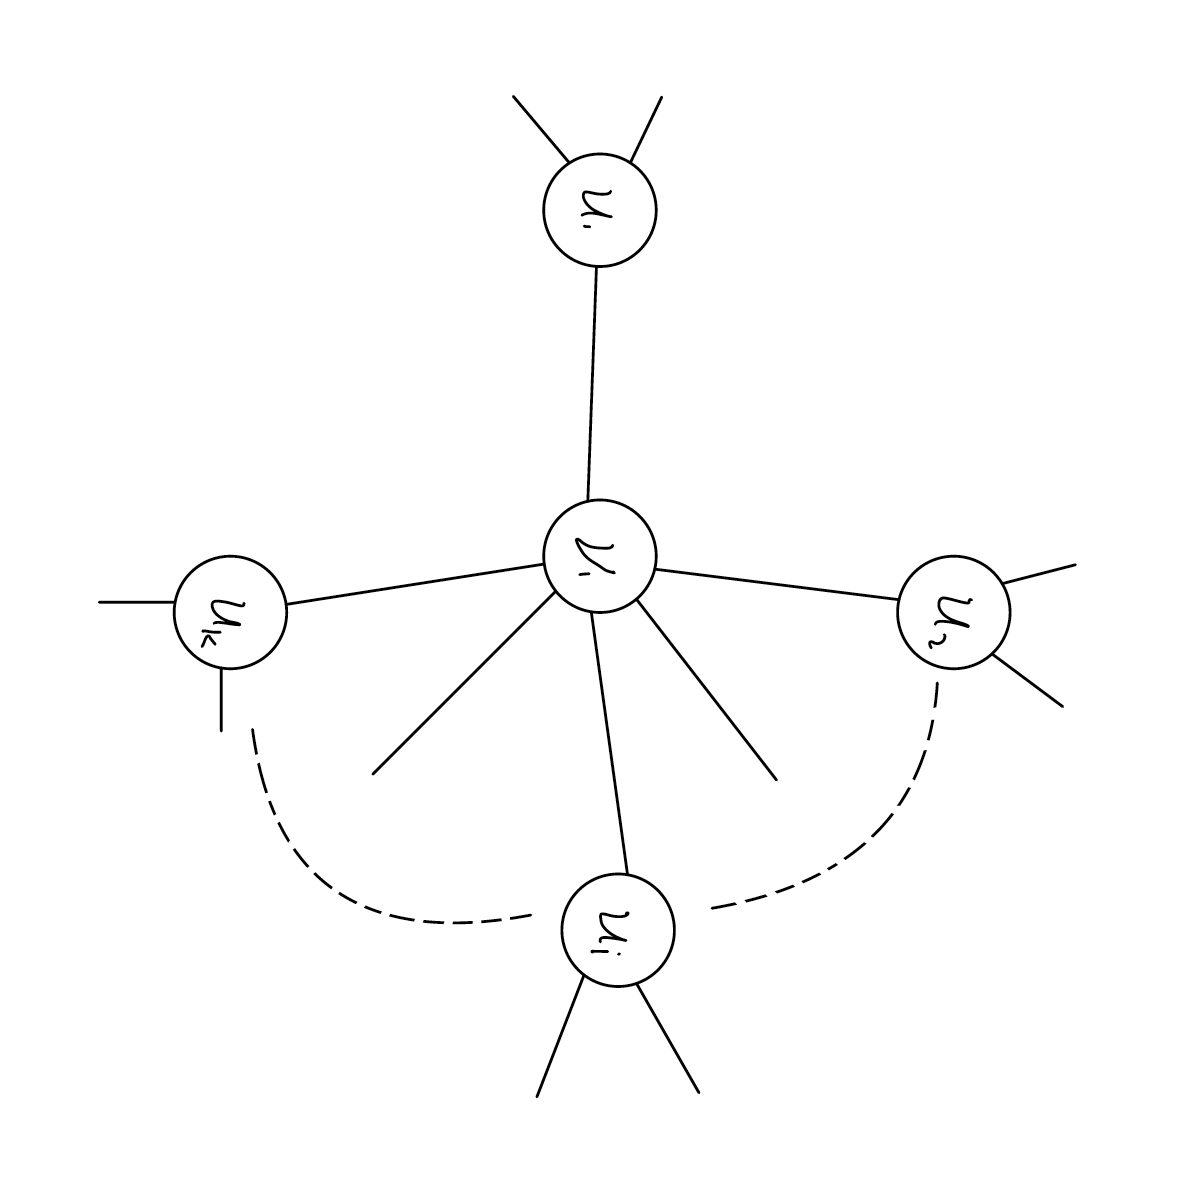
\includegraphics[width=\linewidth]{figures/kvertex1.png}}
    \caption{a common neighbor}
    \label{fig:kvertex1}
  \end{minipage}
  \begin{minipage}{0.48\linewidth}
    \centering
    \rotatebox{90}{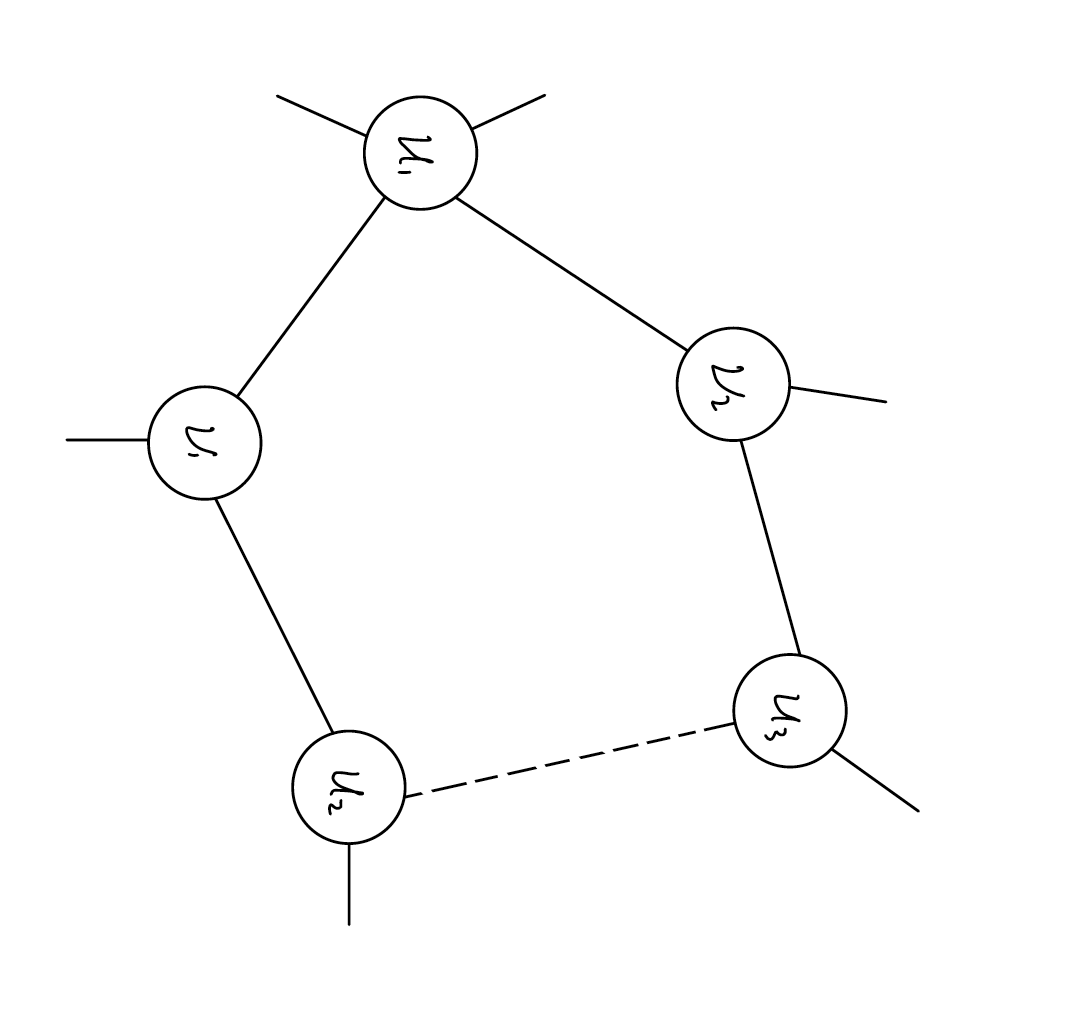
\includegraphics[width=\linewidth]{figures/kvertex2.png}}
    \caption{2-hop neighbors}
    \label{fig:kvertex2}
  \end{minipage}
\end{figure}

However, if $k\geq 3$, "used" status in \autoref{alg:2vertexsort} may no longer be helpful. For a center vertex $u_1$, its 2-hop neighbours $u_2$ and $u_3$ can either be neighbors or not neighbors, as shown in \autoref{fig:kvertex2}.

\begin{framed}
\noindent\textbf{Theorem 4.3:}

If a set of $k$ vertices $\{u_1, u_2, \cdots, u_k\}$ is added into $MWIS(G)$ by $k$-vertex reduction $(k\geq 2)$, then it holds that $\forall u_i$, $i\in\{1,2,\cdots,k\}$, $\{u_1, \cdots, u_{i-1}, u_{i+1}, \cdots, u_k\}$ must be an independent set of the set $T_i=\{v | v \text{ is }u_i\text{'s 2-hop neighbor}\}$.
\end{framed}

\begin{proof}
By the definition of an independent set, any pair of vertices $(u_i, u_j)\ (i\neq j)$ from $\{u_1, u_2, \cdots, u_k\}$ must not be neighbors; and by theorem 4.2, $\{u_1, u_2, \cdots, u_k\}$ share at least one common neighbor. Therefore, an arbitrary pair of vertices $(u_i, u_j)\ (i\neq j)$ from $\{u_1, u_2, \cdots, u_k\}$ are 2-hop neighbors of each other. Thus the proof is achieved.
\end{proof}

The reduction algorithm is shown as \autoref{alg:kvertex}.

\begin{algorithm}[tbp]
\caption{$k$-vertex Reduction}
\label{alg:kvertex}
%\SetAlgoLined
\begin{algorithmic}
	\STATE   \textbf{Input} A graph $G=(V_G,E_G,\omega)$
        %\vspace*{-.45cm}
	\STATE   \textbf{Output} $S$: a set of vertices in $MWIS(G)$
	\STATE   initialize $S\leftarrow \emptyset$
	\STATE   \textbf{for} each vertex $u\in V_G$ \textbf{do}
	\STATE   \quad $T \leftarrow \emptyset$
	\STATE   \quad \textbf{for} each vertex $v\in N(u)$ \textbf{do}
	\STATE   \quad \quad \textbf{for} each vertex $w\in N(v)$ \textbf{do}
	\STATE   \quad \quad \quad \textbf{if} $e(u,w) \notin E_G$ \textbf{then}
	\STATE   \quad \quad \quad \quad $T \leftarrow T \cup \{w\}$
	\STATE   \quad calculate the maximal independent sets $\mathcal{M}=\{M_1,...,M_a\}$, $M_i \subseteq T$, $i=1,...,a$
	\STATE   \quad sort $\mathcal{M}$ in descending order so that $\omega(M_1)\geq...\geq\omega(M_a)$
	\STATE   \quad \textbf{for} $M_i\in\mathcal{M}$ \textbf{do}
	\STATE   \quad \quad \textbf{if} $\omega(u)+\omega(M_i)\geq \omega(N(u)\cup N(M_i))$ \textbf{then}
	\STATE   \quad \quad \quad $S\leftarrow S\cup\{u\}\cup M_i$
	\STATE   \quad \quad \quad remove $\{u\}$, $M_i$ and $N(u)\cup N(M_i)$ from G
	\STATE   \quad \quad \quad \textbf{break}
\end{algorithmic}
\end{algorithm}

\section{Experimental Support}
% TODO: experiment

\subsection{Experimental Settings}

\noindent\textbf{Graphs}. We tested our algorithm on several graphs at different scales. The graphs are downloaded from \emph{Stanford Network Analysis Platform}~\cite{snapnets} (short as SNAP), \emph{The SuiteSparse Matrix Collection}~\cite{2011The} (short as SSMC) and \emph{The Index of Complex Networks}~\cite{iconnets} (short as ICON). \autoref{tab:graph} lists the statistics.

\begin{table}[htbp]% h asks to places the floating element [h]ere.
  \caption{Statistics of Graphs Used for Experiment}
  \label{tab:graph}
  \begin{tabular}{cccccc}
    \toprule
    \textbf{ID} & \textbf{Graph Name} & \textbf{|V(G)|} & \textbf{|E(G)|} & \textbf{Source} & \textbf{Weight}\\
    \midrule
    G01 & sw-full-inter & 110 & 398 & ICON & original\\
    G02 & GD98\_c & 112 & 168 & SSMC & random\\
    G03 & USAir97 & 332 & 2\,126 & SSMC & random\\
    G04 & ca-GrQC & 5\,242 & 14\,496 & SNAP & random\\
    G05 & ca-AstroPh & 18\,772 & 198\,110 & SNAP & random\\
    G06 & roadNet-PA & 1\,088\,092 & 1\,541\,898 & SNAP & random\\
    G07 & roadNet-CA & 1\,965\,206 & 2\,766\,607 & SNAP & random\\
  \bottomrule
\end{tabular}
\end{table}

These networks are popular benchmark instances commonly used for the maximum independent set problem. However, most of them are unweighted, and comparable weighted instances are very scarce. Therefore, a common approach in literature is to assign vertex weights uniformly at random from a fixed size interval~\cite{2018Improving,2017An}. To keep our results in line with existing work~\cite{Lamm0SWZ19}, we assigned vertex weights uniformly at random from [1, 200].

\noindent\textbf{Algorithms}. 

\noindent\textbf{Metrics}. 

\subsection{Experimental Results}

\section{Conclusion}
% TODO: conclusion

In this paper, we proposed 

% \subsection{Figures}

% Duck \autoref{fig:duck}.

% \begin{figure}
%   \centering
%   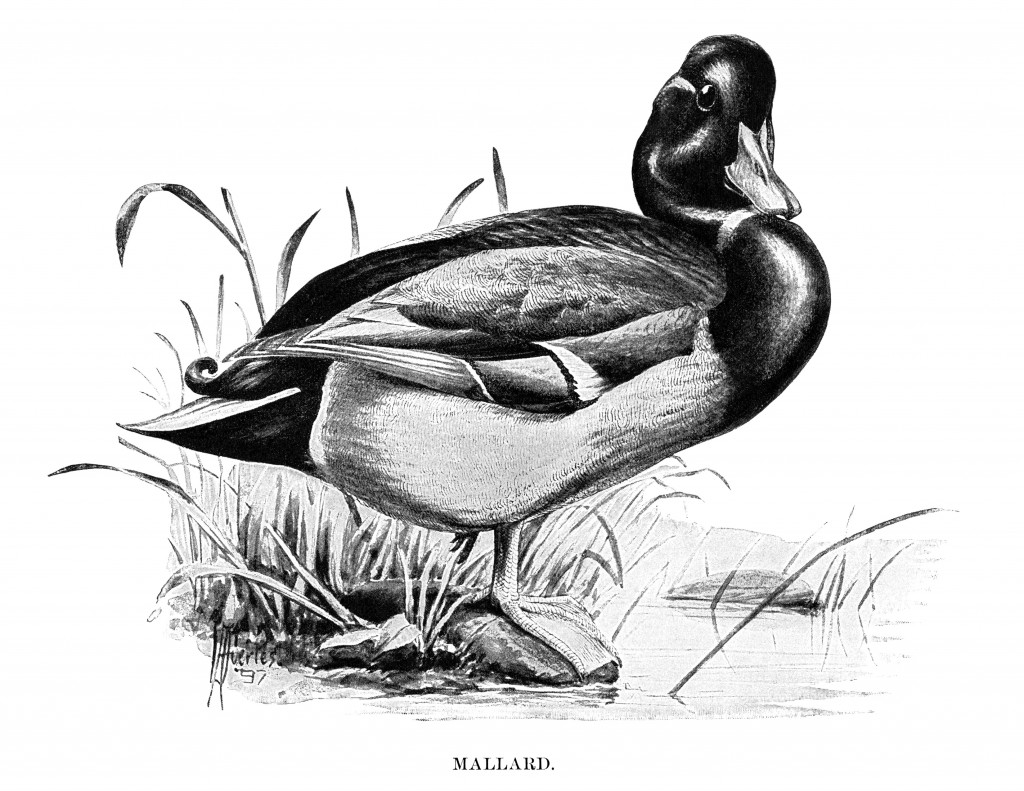
\includegraphics[width=\linewidth]{figures/duck}
%   \caption{An illustration of a Mallard Duck. Picture from Mabel Osgood Wright, \textit{Birdcraft}, published 1897.}
%   \label{fig:duck}
% \end{figure}

% \begin{table*}[t]
%   \caption{A double column table.}
%   \label{tab:commands}
%   \begin{tabular}{ccl}
%     \toprule
%     A Wide Command Column & A Random Number & Comments\\
%     \midrule
%     \verb|\tabular| & 100& The content of a table \\
%     \verb|\table|  & 300 & For floating tables within a single column\\
%     \verb|\table*| & 400 & For wider floating tables that span two columns\\
%     \bottomrule
%   \end{tabular}
% \end{table*}

% \subsection{Tables}

% \begin{table}[hb]% h asks to places the floating element [h]ere.
%   \caption{Frequency of Special Characters}
%   \label{tab:freq}
%   \begin{tabular}{ccl}
%     \toprule
%     Non-English or Math & Frequency & Comments\\
%     \midrule
%     \O & 1 in 1000& For Swedish names\\
%     $\pi$ & 1 in 5 & Common in math\\
%     \$ & 4 in 5 & Used in business\\
%     $\Psi^2_1$ & 1 in 40\,000 & Unexplained usage\\
%   \bottomrule
% \end{tabular}
% \end{table}

% \subsection{Listings and Styles}

% \begin{itemize}
% \item Duis lacinia mollis purus, ac aliquet arcu dignissim ac. Vivamus accumsan sollicitudin dui, sed porta sem consequat.
% \item Curabitur ut mauris vel augue tempor suscipit eget eget lacus. Sed pulvinar lobortis dictum. Aliquam dapibus a velit.
% \item Curabitur vitae nulla dapibus, ornare dolor in, efficitur enim.
% \end{itemize}

% \begin{enumerate}
% \item Duis lacinia mollis purus, ac aliquet arcu dignissim ac. Vivamus accumsan sollicitudin dui, sed porta sem consequat.
% \item Curabitur ut mauris vel augue tempor suscipit eget eget lacus. Sed pulvinar lobortis dictum. Aliquam dapibus a velit.
% \item Curabitur vitae nulla dapibus, ornare dolor in, efficitur enim.
% \end{enumerate}

% \subsection{Math and Equations}

% \begin{equation}
%   \lim_{n\rightarrow \infty}x=0
% \end{equation}
 
% \begin{displaymath}
%   \sum_{i=0}^{\infty} x + 1
% \end{displaymath}

% \begin{equation}
%   \sum_{i=0}^{\infty}x_i=\int_{0}^{\pi+2} f
% \end{equation}

%==========

\begin{acks}
% This work was supported by the [...] Research Fund of [...] (Number [...]). Additional funding was provided by [...] and [...]. We also thank [...] for contributing [...].
This work was the coursework of course \emph{Graph Data Management and Mining} (No. DATA130045.01) at Fudan University.
\end{acks}

% \clearpage

\bibliographystyle{ACM-Reference-Format}
\interlinepenalty=10000
%\bibliography{sample}
\bibliography{reference}

\end{document}
\endinput
